\section{Quantum Approximate Optimization Algorithm}
\label{Section:QAOA}

The Quantum Approximate Optimization Algorithm (QAOA) is a hybrid quantum-classical algorithm
introduced by Farhi et al.~\cite{farhi_quantum_2014} to tackle combinatorial optimization problems.
Its goal is to approximate the ground state of a cost Hamiltonian whose minimum encodes the
optimal solution to the problem. QAOA is particularly suited to near-term quantum devices
due to its shallow circuit depth and iterative variational structure, which offloads part
of the computational workload to a classical optimizer.

At its core, QAOA constructs a parametrized quantum state (ansatz) by sequentially applying
two alternating types of unitaries derived from two Hamiltonians:
\begin{itemize}
    \item The cost Hamiltonian $H_C$, which encodes the objective function of the optimization
    problem. This is typically written in the form of an Ising Hamiltonian.
    \item The mixing Hamiltonian $H_M$, which introduces transitions between computational
    basis states to enable exploration of the solution space. A common choice is:
    \begin{equation}
        H_M = \sum_i \sigma_i^x,
        \label{eq:mixing_hamiltonian}
    \end{equation}
    where $\sigma_i^x$ is the Pauli-X operator acting on qubit $i$.
\end{itemize}

The algorithm starts with the initial state $\ket{\psi_0} = \ket{+}^{\otimes n}$, which is
the ground state of $H_M$ and a uniform superposition over all computational basis states.
The QAOA ansatz with $p$ layers is constructed as:
\begin{equation}
    \ket{\psi_p(\bm{\gamma}, \bm{\beta})} = e^{-i \beta_p H_M} e^{- i \gamma_p H_C} \cdots
    e^{-i \beta_1 H_M} e^{- i \gamma_1 H_C} \ket{+}^{\otimes n},
    \label{eq:qaoa_state_evolution}
\end{equation}
where $\bm{\gamma} = (\gamma_1, \dots, \gamma_p)$ and $\bm{\beta} = (\beta_1, \dots, \beta_p)$
are real variational parameters to be optimized.

The performance of a QAOA instance is assessed by evaluating the expected value of the cost
Hamiltonian in the ansatz state:
\begin{equation}
    F_p (\bm{\gamma}, \bm{\beta}) = \bra{\psi_p (\bm{\gamma}, \bm{\beta})} H_C \ket{\psi_p (\bm{\gamma}, \bm{\beta})}.
    \label{eq:cost_function}
\end{equation}
This expectation value serves as the cost function for the classical optimizer. The parameters $(\bm{\gamma}, \bm{\beta})$ are iteratively updated to minimize $F_p$, with quantum circuits being re-evaluated at each step until convergence.

\begin{figure}[h]
    \centering
    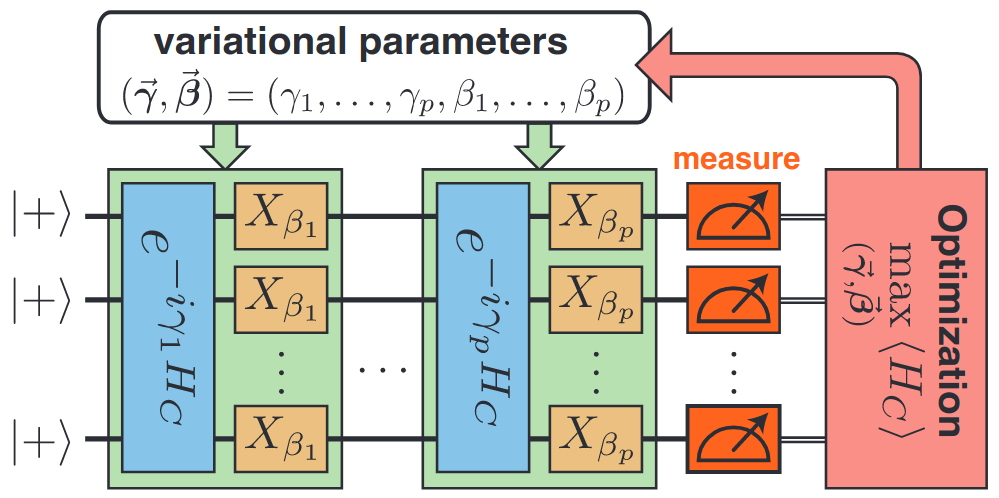
\includegraphics[width=0.6\textwidth]{01-introduction/figs/qaoa.png}
    \caption{Diagram of a $p$-layer QAOA circuit. Starting from the initial state $\ket{+}^{\otimes n}$,
    the circuit alternates between applying the unitaries $e^{-i \gamma_i H_C}$ and $e^{-i \beta_i H_M}$
    for $i = 1$ to $p$. The final state is measured to estimate the expectation value $\langle H_C \rangle$,
    which is passed to a classical optimizer. This process is repeated until convergence.}
    \vspace{0.3em}
    \small\textit{Source: Adapted from Zhou et al., 2019.}
    \label{fig:qaoa}
\end{figure}

The QAOA stands out as one of the most compelling candidates for demonstrating quantum advantage
on near-term quantum devices. From a complexity-theoretic standpoint, Farhi et al.~\cite{farhi_quantum_2019}
argue that sampling from the output distribution of even the lowest-depth version of QAOA (i.e., $p=1$)
could be classically intractable. Specifically, they show that there exist problem instances
and choices of parameters $(\bm{\gamma}, \bm{\beta})$ for which classical algorithms cannot
feasibly reproduce the output of a quantum device running QAOA, strengthening the case for
using it as a path to quantum supremacy.

Beyond theoretical hardness arguments, QAOA also exhibits practical advantages in terms of
implementability and flexibility. Ho and Hsieh~\cite{ho_efficient_2019} introduce a closely
related variational framework (VQCS), which shares the QAOA structure of alternating unitaries
generated by simple Hamiltonians. They demonstrate that such protocols can efficiently prepare
complex, non-trivial quantum states and are compatible with current quantum hardware platforms
such as trapped ions and superconducting qubits. The minimal requirement of time evolution
under simple, local Hamiltonians makes QAOA especially attractive for near-term experimental
implementation.

Additionally, the adaptability of QAOA makes it suitable for a wide variety of problem domains,
including factoring. In their work on Variational Quantum Factoring (VQF), Anschuetz et
al.~\cite{anschuetz_variational_2018} apply a QAOA-like approach to integer factorization,
showing that hybrid quantum-classical heuristics can offer a path toward solving classically
hard problems on noisy intermediate-scale quantum (NISQ) devices. While challenges
remain particularly related to scalability and robustness against noise the framework's
modularity and reliance on classical feedback make it well-suited for real-world NISQ conditions.